\documentclass[11pt,a4paper]{article} 

\usepackage[T1]{fontenc}
\usepackage[utf8]{inputenc}
\usepackage{lmodern}
\usepackage[french,english]{babel}

\usepackage{amsthm}
\usepackage{float}
\usepackage{lmodern}%pour un meilleur rendu des polices
\usepackage{verbatim}%du texte non interprt
\usepackage[cmex10]{amsmath}
\usepackage{amssymb}%maths
\usepackage{xspace}
\usepackage[dvipsnames,svgnames,table]{xcolor}
\usepackage{listings}
\usepackage{fancyhdr}
\usepackage{etoolbox}
\usepackage{titlesec}
\usepackage{titletoc}
\usepackage{lastpage}
\usepackage[bookmarks=true,bookmarksnumbered=true]{hyperref}
\usepackage{ctable} % for \specialrule command
\usepackage{cite}
\usepackage{algorithm2e}
\usepackage{alltt}
\usepackage{array}
\usepackage{mdwmath}
\usepackage{mdwtab}
\usepackage{eqparbox}
\usepackage[caption=false,font=normalsize,labelfont=sf,textfont=sf]{subfig}
\usepackage{dblfloatfix}
\usepackage{url}
\usepackage{tipa}
\usepackage{stmaryrd}
\usepackage{mathrsfs}
\usepackage{ulem}

%\usepackage{natbib}
%\usepackage[pdftex]{graphicx}
%\usepackage{framed}
%\usepackage[usenames]{color}

\graphicspath{{img/}}
\DeclareGraphicsExtensions{.pdf,.jpeg,.jpg,.png}

%% taille du papier
\textwidth 16 true cm
\textheight 24 true cm
\addtolength{\hoffset}{-1.5cm}
\addtolength{\voffset}{-1.5cm}

%-------- couleurs
\definecolor{grisf}{rgb}{.47,.47,.47} % barre de droite gris fonce
\definecolor{imag}{RGB}{50,0,100}
\definecolor{darkimag}{RGB}{65,15,100}
\definecolor{darkgreen}{RGB}{65,15,100}
\newcommand{\colorc}{\color{darkimag}}
\newcommand{\colorb}{\color{darkimag}}
\newcommand{\colora}{\color{Blue}}

%----------- sections et TOC
% chapitres
\titleformat{\chapter}[display]
  {\normalfont\sffamily\bfseries\huge\colora\centering}{\thechapter}{1ex}
  {{\titlerule[1pt]}\vspace{1.3ex}}[\vspace{1ex}{{\titlerule[1pt]}}]
  
% chapitres etoiles  
\titleformat{name=\chapter,numberless}[display]
  {\normalfont\sffamily\bfseries\LARGE\colora\centering}{}{1ex}
  {{\titlerule[1pt]}\vspace{1.3ex}}[\vspace{1ex}{\titlerule[1pt]}\vspace{2ex}]
  
% sections  
\titleformat{\section}[hang]{\Large\normalfont\sffamily\bfseries\colora}{{\thesection\, }}{0 em}
  {}[{\titlerule[1pt]}\vspace{1ex}]

  
% sous section, sous sous sec, paragraphes  
\titleformat{\subsection}[hang]{\Large\normalfont\sffamily\bfseries\colorc}{{\thesubsection\, }}{0 em}
  {}[{\titlerule}\vspace{.7ex}]
\titleformat{\subsubsection}[hang]{\normalfont\sffamily\bfseries\large}{{\thesubsubsection\, }}{0 em}
  {}[{\color{grisf}\titlerule}\vspace{3pt}]
\titleformat{\paragraph}[runin]{\normalfont\sffamily\bfseries\colorb}{}{0 em}
  {\indent}



%----------------- fancy headers -------------%

\makeatletter
\patchcmd{\@fancyhead}{\rlap}{\color{grisf}\rlap}{}{}
\patchcmd{\headrule}{\hrule}{\color{grisf}\hrule}{}{}
\patchcmd{\@fancyfoot}{\rlap}{\color{grisf}\rlap}{}{}
\patchcmd{\footrule}{\hrule}{\color{grisf}\hrule}{}{}
\makeatother

                                                                    
\fancyhf{}
\fancyhead[R]{\sffamily\colorb{Report}}
\fancyfoot[R]{\sffamily\small\colorb{\thepage/\pageref{LastPage}}}
\fancyhead[L]{\sffamily\small\colorb{Jean-Baptiste Keck}}
\fancyfoot[L]{\sffamily\small\colorb{M2 MSIAM -- Inverse Methods -- 2014-2015}}
\renewcommand{\headrulewidth}{0.2pt} %0.4
\renewcommand{\footrulewidth}{0.2pt} %0
\addtolength{\headheight}{0.pt}

\fancypagestyle{plain}{
  \fancyhead{}
  \renewcommand{\headrulewidth}{0pt}
  }
     
  %-- macros --%   
  \def\hlinewd#1{%
      \noalign{\ifnum0=`}\fi\hrule \@height #1 %
  \futurelet\reserved@a\@xhline} 

  
  
  %------------------- front page ------------------%
  \title{
      \bsc{TP Inverse Methods}
      \vskip 1cm
      {\colorb\textbf{Lorenz Attractor}}
      \vskip 1cm
      \colorb\textit{Report}
  }
\author{%
    Jean-Baptiste \bsc{Keck}
    \vskip 0.5cm
    \bsc{M2 Msiam}
}
%\date{27 janvier 2014}
\makeatletter

\def\maketitle{%
    %\thispagestyle{empty}%
    \begin{flushleft}
        \normalfont\LARGE\par
    \end{flushleft}
    \vskip 3cm
    \begin{center}%
        {\colora\specialrule{.2em}{0em}{0em}}
        \vskip 1cm
        {\Huge \@title}%
        \vskip 1cm
        {\colora\specialrule{.2em}{0em}{0em}}
        \vskip 5cm
        {\Huge \@author\par}%
        \vskip 2cm
        {\Huge \@date\par}%
        \vskip 1cm

    \end{center}%
    \clearpage
}

\renewcommand{\ccite}[1]{\textbf{\cite{#1}}}
\renewcommand{\pd}[2]{\dfrac{\partial #1}{\partial #2}}
\renewcommand{\abs}[1]{\left( #1 \right)}
\renewcommand{\norm}[1]{\lVert #1 \rVert}
\renewcommand{\dx}{\ \mathrm{d}x}
\renewcommand{\dt}{\ \mathrm{d}t}
\renewcommand{\u} {\mathbf{u}}
\renewcommand{\k} {\mathbf{k}}
\renewcommand{\v} {\mathbf{v}}
\renewcommand{\w} {\mathbf{w}}
\renewcommand{\h} {\mathbf{h}}
\renewcommand{\f} {\mathbf{f}}
\renewcommand{\g} {\mathbf{g}}
\renewcommand{\uz}{\mathbf{u_0}}
\renewcommand{\ud}{\mathring{\mathbf{u}}}
\renewcommand{\ut}{\tilde{\mathbf{u}}}
\renewcommand{\utrue}{\mathbf{u}^t}}
\renewcommand{\uobs}{\mathbf{u}^{obs}}}
\renewcommand{\xobs}{x^{obs}}}
\renewcommand{\utz}{\tilde{\mathbf{u}}_0}
\renewcommand{\uh}{\hat{\mathbf{u}}}
\renewcommand{\vh}{\hat{\mathbf{v}}}
\renewcommand{\wh}{\hat{\mathbf{w}}}
\renewcommand{\ub}{\bar{\mathbf{u}}}
\renewcommand{\F}{\mathrm{F}}
\renewcommand{\R}{\mathbb{R}}
\renewcommand{\J}{\mathcal{J}}
\renewcommand{\xt}{\tilde{x}}
\renewcommand{\xh}{\hat{x}}
\renewcommand{\yh}{\hat{y}}
\renewcommand{\zh}{\hat{z}}
\renewcommand{\xb}{\bar{x}}

\newcommand{\bigo}[1]{\ensuremath{\mathop{}\mathopen{}O\mathopen{}\left(#1\right)}}
\newcommand{\smallo}[1]{\ensuremath{\mathop{}\mathopen{}o\mathopen{}\left(#1\right)}}

\definecolor{lightgray}{gray}{0.9}
\renewcommand{\colbox}[1]{\colorbox{lightgray}{$ #1 $}}
%%%%%%%

\begin{document}
\pagestyle{fancy}

\maketitle

\clearpage
\tableofcontents
\clearpage

\section{Theoretical work on the continuous model}

\textbf{Lorentz Equations :}
\vskip 0.2cm

$$
\begin{equation} \label{eq:lorentz}
\left \{
\begin{array}{l c l}
    \mathring{x} & = & 10(y - x)\\
    \mathring{y} & = & 28x - y -xz\\
    \mathring{z} & = & xy - \frac{8}{3}z\\
    \multicolumn{3}{l}{x(0) = x_0,\ y(0) = y_0,\ z(0) = z_0}
\end{array}
\right .
\hskip 0.5cm
\Leftrightarrow 
\hskip 0.5cm
\colbox{
\left \{
\begin{array}{l c l}
\ud&=&\f(\u) \\
\u_0&=&[x_0, y_0, z_0]^T
\end{array}
\right .
}
\end{equation}
$$

with $\u(t) = 
\left [
    \begin{array}{c}
        x(t)&
        y(t)&
        z(t)
    \end{array}
\right ]$
and $\f(\u) =
\left [
    \begin{array}{c}
        10(y - x)\\
        28x - y -xz\\
        xy - \frac{8}{3}z\\
    \end{array}
\right ]
$

\vskip 0.5cm
\subsection{Question 1:} 

\vskip 0.3cm
\noindent Let $\J$ be the following cost function :
\vskip 0.3cm

$\colbox{\J(\u_0) = \dfrac{1}{2}\displaystyle \int_0^T\norm{\u(t)-\uobs(t)}^2 \dt}$ where $\u$ is the solution of (1) with initial condition $\u_0$.

\vskip 0.5cm
\noindent Let $T \in \R^*_+,\ \alpha \in \R^*,\ \u_0 \in \R^3,\ \delta\u_0 \in \R^3$
and
$\ut_0 = \u_0 + \alpha\ \delta\u_0$.
\vskip 0.1cm
\noindent Let $\u$ (resp. $\ut$) be the unique solution of the system (\ref{eq:lorentz}) with $\u_0$ (resp. $\ut_0$) as initial condition.
\vskip 0.1cm
\noindent Let $\ub = \dfrac{\ut - \u}{\alpha}$,  $\uh = \lim\limits_{\alpha \to 0} \ub$
}
and assume 
$\mathrm{K} = \left\{t \in\ ]0,T[\ \ |\ \ \norm{\uh(t)} = +\infty \right\}$
is a measure-zero set.
\vskip 0.5cm

$$
\begin{equation} \label{eq:grad}
    \colbox{
        d\left(\J(\u_0)\right)(\delta \u_0) 
        =\nabla \J(\u_0) \cdot \delta\u_0
        = \lim\limits_{\alpha \to 0}\dfrac{\J(\ut_0) - \J(\u_0)}{\alpha}\ 
    }
\end{equation}
$$

$
\mathcal{J}_\alpha
=\dfrac{\J(\utz) - \J(\uz)}{\alpha}
= \dfrac{1}{2\alpha}\displaystyle \int_0^T \left[ \norm{\ut(t) - \uobs(t)}^2 - \norm{\u(t)-\uobs(t)}^2 \right ] \dt
\vskip 0.2cm
\hskip 3.75cm
=\dfrac{1}{2\alpha}\displaystyle \int_0^T \left[ \norm{\u(t) - \uobs(t) + \alpha\ \ub(t)}^2 - \norm{\u(t)-\uobs(t)}^2 \right ] \dt
\vskip 0.2cm
\hskip 3.75cm
=\dfrac{1}{2\alpha}\displaystyle \int_0^T \left[ \alpha^2\ \norm{\ub(t)}^2 + 2 \langle \u(t) - \uobs(t), \alpha\ \ub(t) \rangle\right] \dt
\vskip 0.2cm
\hskip 3.75cm
=\dfrac{1}{2}\displaystyle \int_0^T \left[ \alpha\ \norm{\ub(t)}^2 + 2 \langle \u(t) - \uobs(t), \ub(t) \rangle\right] \dt
\vskip 0.2cm
\hskip 3.75cm
$

$
\Rightarrow
d\left(\J(\u_0)\right)(\delta \u_0) 
= \lim\limits_{\alpha \to 0} \mathcal{J}_\alpha
= \lim \limits_{\alpha \to 0} \dfrac{1}{2}\displaystyle \int_0^T \left[ \alpha\ \norm{\ub(t)}^2 + 2 \langle \u(t) - \uobs(t), \ub(t) \rangle\right] \dt
\vskip 0.2cm
\hskip 3.2cm
= \lim \limits_{\alpha \to 0} 
\left [ \dfrac{1}{2}\displaystyle  \int_{]0,T[ \backslash K} \alpha\ \underbrace{\norm{\ub(t)}^2}_{\leq M} \dt \right ]
+ \displaystyle \int_0^T \langle \u(t) - \uobs(t), \uh(t) \rangle \dt
\vskip 0.2cm
\hskip 3.2cm
= 0 + \displaystyle \int_0^T \langle \u(t) - \uobs(t), \uh(t) \rangle \dt
$

\vskip 0.2cm
$$
\begin{equation} \label{eq:diff}
\colbox{
d\left(\J(\u_0)\right)(\delta \u_0) 
= \displaystyle \int_0^T \left[ \u(t) - \uobs(t) \right]^T \uh(t) \dt
}
\end{equation}
$$

\noindent\textbf{Tangent model :} 

\vskip 0.2cm
$
\widetilde{(1)} - (1) 
\Leftrightarrow
\left \{
\begin{array}{l c l}
    \mathring{\ut} - \mathring{\u} &=&\f(\ut) - \f(\u)\\
    \ut(0) - \u(0)&=&\ut_0 - \u_0
    \right .
\end{array}
\right.
\vskip 0.2cm
\hskip 1.55cm
\Leftrightarrow
\left \{
\begin{array}{l c l}
    \alpha\ \mathring{\ub} &=& \f(\u + \alpha \ub) - \f(\u)\\
    \alpha \ub(0)&=&\alpha\ \delta \u_0
    \right .
}
\end{array}
\right.
\vskip 0.2cm
\hskip 1.55cm
\Rightarrow
\left \{
\begin{array}{l c l c l c l}
    \mathring{\uh} &=&
    \lim\limits_{\alpha \to 0}  \dfrac{\f(\u + \alpha \ub) - \f(\u)}{\alpha}&=&
    d(\f(\u))(\uh) = J_f(\u)\ \uh\\
    \uh(0)&=&\delta \u_0&&
    \right .
}
\end{array}
$

$$
\begin{equation} \label{eq:tangent}
\colbox{
\left \{
\begin{array}{l c l}
    \pd{\uh}{t} &=&J_f(\u)\ \uh\\
    \uh(0)&=&\delta \u_0
    \right .
\end{array}
}
\textrm{ with }
\colbox{
    J_f(\u) = \pd{\f}{\u}(\u) = 
\left [
    \begin{array}{c c c}
        -10&10&0\\
        28-z&-1&-x\\
        y&x&-\frac{8}{3}
    \end{array}
\right ]
}
\end{equation}
$$

\noindent\textbf{Adjoint model :} 
\vskip 0.2cm

Let $\vh :\ ]0,T[\ \to \R^3$ continuously differentiable.

\hskip 0.7cm
$\uh$ may be continuously differentiable because of (4) under stronger assumptions on K 

\hskip 0.7cm
(see 2), $ie$ K$=\varnothing$.

Commodity notations : $\uh \cdot \vh = \langle \uh, \vh \rangle$ and $\uh' = \pd{\uh}{t}$.

\vskip 0.3cm
By integrating the scalar product by part :

$$
\left[ \vh(t) \cdot \uh(t) \right]_0^T
=
\displaystyle \int_0^T \left[
    \vh'(t) \cdot \uh(t)
    + \vh(t) \cdot \uh'(t)
\right] \dt
$$

$$
\Leftrightarrow
\underbrace{\vh(T)}_{\textrm{set to } \vec{0}} \cdot \uh(T)
-  \vh(0) \cdot \underbrace{\uh(0)}_{\delta\uz}
=
\displaystyle \int_0^T \left[
    \vh'(t) \cdot \uh(t)
    + \underbrace{\vh(t) \cdot J_f(\u(t))\uh(t)}_{J_f^*(\u(t)) \vh(t) \cdot \uh(t)}
\right] \dt
$$

$$
\Leftrightarrow
\begin{equation}
\colbox{
    \displaystyle \int_0^T
    \left[
        \vh'(t) + J_f^*(\u(t)) \vh(t)
    \right ]
    \cdot \uh(t)
\right] \dt
=
-  \vh(0) \cdot \delta\uz
 }
\end{equation}
$$

\vskip 0.5cm
Knowing $\u(t)$ and $\uobs(t)\ \forall t\in [0,T]$, and if we take $\vh$ solution of the following adjoint model:

$$
\begin{equation} \label{eq:adjoint}
\hskip 0.5cm
\colbox{
\left \{
\begin{array}{l c l}
    \mathring{\vh}&=&\g(\vh,t) + \h(t)\\
    \vh(T)&=&\vec{0}
\end{array}
\right .
}
\textrm{ with }
\left \{
\begin{array}{l l l l l}
\g(\vh,t)&=&-J_f^*(\u(t))\ \vh(t)&=&-J_f^T(\u(t))\ \vh(t)\\
\h(t)&=&\u(t) - \uobs(t)
\end{array}
\right .
\end{equation}
$$

By (2), (3) and (5) we get directly $\colbox{\nabla \J(\uz) = - \vh(0)}$.





\vskip 0.5cm
\subsection{Question 2:} 
\vskip 0.3cm
\noindent Let now $\J_x$ be the following cost function :
\vskip 0.3cm

$\colbox{\J_x(\u_0) = \dfrac{1}{2}\displaystyle \int_0^T\abs{x(t)-\xobs(t)}^2 \dt}$ where $x$ is the solution of (1) projected on the x-axis with initial condition $\u_0$.

\vskip 0.5cm
With the same notations and assumptions as before on $x$ :

$$
\begin{equation} \label{eq:grad}
    \colbox{
        d\left(\J_x(\u_0)\right)(\delta \u_0) 
        =\nabla \J_x(\u_0) \cdot \delta\u_0
        = \lim\limits_{\alpha \to 0}\dfrac{\J_x(\ut_0) - \J_x(\u_0)}{\alpha}\ 
    }
\end{equation}
$$

$
\mathcal{J}_x^\alpha
=\dfrac{\J(\utz) - \J(\uz)}{\alpha}
= \dfrac{1}{2\alpha}\displaystyle \int_0^T \left[ \abs{\xt(t) - \xobs(t)}^2 - \abs{x(t)-\xobs(t)}^2 \right ] \dt
\vskip 0.2cm
\hskip 3.75cm
=\dfrac{1}{2\alpha}\displaystyle \int_0^T \left[ \abs{x(t) - \xobs(t) + \alpha\ \xb(t)}^2 - \abs{x(t)-\xobs(t)}^2 \right ] \dt
\vskip 0.2cm
\hskip 3.75cm
=\dfrac{1}{2\alpha}\displaystyle \int_0^T \left[ \alpha^2 \xb(t)^2 + 2\alpha\ [x(t) - \xobs(t)]\ \xb(t) \right] \dt
\vskip 0.2cm
\hskip 3.75cm
=\dfrac{1}{2}\displaystyle \int_0^T \left[ \alpha \xb(t)^2 + 2\ [x(t) - \xobs(t)]\ \xb(t) \right] \dt
\vskip 0.2cm
\hskip 3.75cm
$

$
\Rightarrow
d\left(\J_x(\u_0)\right)(\delta \u_0) 
= \lim\limits_{\alpha \to 0} \mathcal{J}_x^\alpha
= \lim \limits_{\alpha \to 0} \dfrac{1}{2}\displaystyle \int_0^T \left[ \alpha\ \xb(t)^2 + 2\ [x(t) - \xobs(t)]\ \xb(t) \right] \dt
\vskip 0.2cm
\hskip 3.2cm
= \lim \limits_{\alpha \to 0} 
\left [ \dfrac{1}{2}\displaystyle  \int_{]0,T[ \backslash K_x} \alpha\ \underbrace{\xb(t)^2}_{\leq M} \dt \right ]
+ \displaystyle \int_0^T [x(t) - \xobs(t)]\ \xh(t) \dt
\vskip 0.2cm
\hskip 3.2cm
= 0 + \displaystyle \int_0^T [x(t) - \xobs(t)]\ \xh(t) \dt
$

\vskip 0.2cm
$$
\begin{equation} \label{eq:diff}
\colbox{
d\left(\J_x(\u_0)\right)(\delta \u_0) 
= \displaystyle \int_0^T [x(t) - \xobs(t)]\ \xh(t) \dt
}
\end{equation}
$$

\noindent\textbf{Tangent model :} 

\vskip 0.2cm
We still have the same tangent model as before (4), and we can project the equations on $x$, $y$ and $z$ to obtain :

$$
\begin{equation} \label{eq:tangent}
    \colbox{
        \left \{
            \begin{array}{l c l}
                \pd{\xh}{t} &=&\pd{f_x}{\u}(\u)\cdot \uh\\
                \\
                \pd{\yh}{t} &=&\pd{f_y}{\u}(\u)\cdot \uh\\
                \\
                \pd{\zh}{t} &=&\pd{f_z}{\u}(\u)\cdot \uh\\
                \\
                \uh(0)&=&\delta \u_0
            \end{array}
        \right .
        \textrm{ with }
        \left\{
                \begin{array}{c c c c l c c c l}
                    \pd{f_x}{\u}(\u)&=&\nabla f_x(\u)&=& [-10 & 10 & 0]^T\\
                    \\
                    \pd{f_y}{\u}(\u)&=&\nabla f_y(\u)&=& [28-z & -1 & -x]^T\\
                    \\
                    \pd{f_z}{\u}(\u)&=&\nabla f_z(\u)&=& [y & x & -\frac{8}{3}]^T\\
                \end{array}
        \right .
    }
\end{equation}
$$

\noindent\textbf{Adjoint model :} 
\vskip 0.2cm

If we take a new function $\wh$ and we integrate the scalar product by part, we still get (5) :

$$
\colbox{
\displaystyle \int_0^T 
\left[ 
    \wh'(t) + J_f^*(\u(t)) \wh(t) 
\right ]
\cdot \uh(t)
\right] \dt
=
-  \wh(0) \cdot \delta\uz
}
$$

\vskip 0.5cm
Knowing $\u(t)$ and $\uobs(t)\ \forall t\in [0,T]$, and if we take $\wh$ solution of the following adjoint model:

$$
\begin{equation} \label{eq:adjoint}
\hskip 0.5cm
\colbox{
\left \{
\begin{array}{l c l}
    \mathring{\wh}&=&\g(\wh,t) + \h^x(t)\\
    \wh(T)&=&\vec{0}
\end{array}
\right .
}
\textrm{ with }
\left \{
\begin{array}{l l l l l}
    \g(\wh,t)&=&-J_f^*(\u(t))\ \wh(t)&=&-J_f^T(\u(t))\ \wh(t)\\
    \h^x(t)&=&\left[ x(t) - \xobs(t), 0, 0 \right]^T
\end{array}
\right .
\end{equation}
$$

The only thing that changed in the adjoint model is the expression of $h(t)$, the new adjoint model does no more take into account the distance between $y$ and $y^{obs}$ or $z$ and $z^{obs}$.
With this new adjoint model, we still have the same expression for the gradient : $\colbox{\nabla \J_x(\uz) = - \wh(0)}$.


\vskip 0.5cm
\subsection{Question 3:} 
\vskip 0.3cm
\noindent Let finally $\J_2$ be the following cost function :
\vskip 0.3cm

$\colbox{\J_2(\u_0) = \J_b(\u_0) + \J_1(\u_0) 
= \dfrac{1}{2}\norm{\uz - \u^b}^2
+ \displaystyle \int_0^T\norm{\u(t)-\uobs(t)}^2 \dt}$

where $\u$ is the solution of (1) with initial condition $\u_0$ and $\u^b \in \R^3$.

\vskip 0.5cm
\noindent\textbf{Expression of the gradient :} we directly have 
$\colbox{
\nabla \J_2 
= \nabla \J^b + \nabla \J_1
}$
and $\colbox{\nabla \J^b(\uz) = \uz - \u^b}$.
\vskip 0.5cm
\noindent\textbf{Tangent model :} As before nothing changes.
\vskip 0.5cm
\noindent\textbf{Adjoint model :} If $\vh$ is solution of the first adjoint model (6), $\uz - \u^b - \vh(0)$ is the gradient we are looking for because we have seen that $\nabla \J_1(\uz) = -\vh(0)$.

\vskip 0.2cm
\noindent Let $\colbox{\hat{\nu} = \vh + \u^b - \uz}$, we have $\colbox{\mathring{\hat{\nu}} = \mathring{\vh}}$ and $\colbox{-\hat{\nu}(0) = \nabla \J_2(\uz)}$.
\vskip 0.2cm
\noindent As $\g(\vh,t)$ is linear in $\vh$ we can easily get the new adjoint model verified by $\hat{\nu}$ :

$$
\begin{equation} \label{eq:adjoint}
\hskip 0.5cm
\colbox{
\left \{
\begin{array}{l c l}
    \mathring{\hat{\nu}}&=&\g(\hat{\nu},t) + \h^b(t)\\
    \hat{\nu}(T)&=&u^b - u_0
\end{array}
\right .
}
\textrm{ with }
\left \{
\begin{array}{l l l}
    \g(\hat{\nu},t)&=&-J_f^*(\u(t))\ \hat{\nu}(t)=-J_f^T(\u(t))\ \hat{\nu}(t)\\
    \h^b(t)&=& u(t) - \uobs(t) + J_f^*(\u(t))\ \left[ \u^b - \uz \right]
\end{array}
\right .
\end{equation}
$$

The adjoint model now takes into account the distance between the initial conditions.

\vskip 0.5cm
\subsection{Question 4:} 
\vskip 0.5cm

Let $\Delta_t > 0,\ \ T = N\Delta_t$ and $\u_k = \left[x_k, y_k, z_k\right]^T$ be the state of the system at time $i\Delta_t\ \forall k \in \llbracket 0,N \rrbracket$. The same notations are used for $\u^{obs}$.

\noindent As $(1)$ is an hyperbolic system, there is a need for high order algorithms like Runge-Kutta 4 (RK4): 

\vskip 0.5cm
\noindent\textbf{Algorithm (RK4):}
\vskip 0.1cm

$\colbox{\u_0 = \u(0)}$\\
\vskip 0.1cm
\indent for k from $0$ to $N-1$:\\
\vskip 0.1cm
\hskip 0.5cm
$
\colbox{
\left [
\begin{array}{l l}
    \u_k^0 = \u_k&
    \k_1 = f(\u_k^0)& 
    \u_k^1 = \u_k + \frac{\Delta_t}{2} \k_1&
    \k_2 = f(\u_k^1)& 
    \u_k^2 = \u_k + \frac{\Delta_t}{2} \k_2&
    \k_3 = f(\u_k^2)&
\u_k^3 = \u_k + \Delta_t \k_3&
    \k_4 = f(\u_k^3)&
    \multicolumn{2}{l}{\u_{k+1} = \u_k + \dfrac{\Delta_t}{6}\left[ \k_1 + 2\k_2 + 2\k_3 + \k_4 \right]}&
\end{array}
\right.
}
$

\vskip 0.5cm
\noindent Let $F(\u) : \R^3 \to \R^{3 \times 3}$ such that $\colbox{f(\u) = F(\u)\u}$ and we denote $\colbox{F_k^l = F(\u_k^l)}$.

\vskip 0.3cm
\noindent As $F$ is not unique, we fix it as 
$
\colbox{
F(\u) = 
\left [
    \begin{array}{c c c}
        -10 & 10 & 0 &
        28-\frac{z}{2} & -1 & -\frac{x}{2}& 
        \frac{y}{2} & \frac{x}{2} & -\frac{8}{3}
    \end{array}
\right ]
}
$

\vskip 0.5cm
\noindent With those notations, one step of (RK4) is equivalent to :

\vskip 0.4cm
\hskip 0.5cm
$
\left [
\begin{array}{l l}
    \u_k^0 = \u_k&
    \k_1 = F_k^0 \u_k^0& 
    \u_k^1 = \u_k + \frac{\Delta_t}{2} \k_1&
    \k_2 = F_k^1 \u_k^1& 
    \u_k^2 = \u_k + \frac{\Delta_t}{2} \k_2&
    \k_3 = F_k^2 \u_k^2& 
\u_k^3 = \u_k + \Delta_t} \k_3&
    \k_4 = F_k^3 \u_k^3& 
    \multicolumn{2}{l}{\u_{k+1} = \u_k + \dfrac{\Delta_t}{6}\left[ \k_1 + 2\k_2 + 2\k_3 + \k_4 \right] = [I + \Delta_tA_k]\u_k} = M_k \u_k&
\end{array}
\right.
$

\vskip 0.3cm
\noindent As I failed to expand $A_k$ by hand, I used maple to get the following \sout{nice and compact} expression:
\begin{multline}
A_k = \dfrac{1}{24} \left[ 
    \Delta_t^3\ F_k^3 F_k^2 F_k^1 F_k^0 
    + 2 \Delta_t^2\left( F_k^3 F_k^2 F_k^1 + F_k^2 F_k^1 F_k^0 \right) 
    + 4 \Delta_t^1\left( F_k^3 F_k^2 + F_k^2 F_k^1 + F_k^1 F_k^0 \right)\\
    + 4 \left( F_k^3 + F_k^0 \right) 
+ 8 \left( F_k^2 + F_k^1 \right) ]
\end{multline}

It can be generated with the maple script $model.mw$. Note that with this expression, computing $M_k$ is much more costly than to compute $u_{k+1}$ directly. The matrix coefficients can be computed analytically with maple but their expression is way to big to fit nicely in this report.

\vskip 0.3cm
We then have $\colbox{M_k = I + \Delta_t A_k}$ and $\colbox{\u_{k+1} = M_k\u_k}$. I checked this matrix form by comparing it to my initial RK4 code and it gave exactly the same results given the $\Delta_t$ powers are applied after all matrix multiplications.

\vskip 0.5cm
\noident At each step $k$ of this algorithm we take into account 4 steps of local linearization on $f$ at intermediate points $x_k^l$, so model error should be taken in account. Let $\colbox{Q_k = Q \in \mathscr{S}_3^{++}}$ be some constant model error covariance matrix.

\vskip 0.5cm
\noident $\colbox{\u_k^{obs} = H_k\mathbf{u}^{t}_k + \mathbf{e}_k}$ are our observations, with $H_k$ the observation matrix. At each step we just directly observe the 3D position of the system in original coordinates so there is no additional transformations and $\colbox{H_k = I}$. We observe those positions with a constant observation error covariance matrix $\colbox{R_k = R \in \mathscr{S}_3^{++}}$.

\vskip 0.5cm
\noident Finally let $\colbox{\u^b = \u_0^t + \epsilon}$ be our approximate initial state with associated covariance matrix $\colbox{P^b \in \mathscr{S}_3^{++}}$. 

\vskip 0.5cm
\noindent \textbf{Kalman Filter Algorithm :}
\vskip 0.5cm

\textbf{Initialization}

\colbox{
$
\begin{array}{l l l l}
    & \u^a_0 & = & \u^b &
    & P^a_0  & = & P^b  &
\end{array}
$
}

\vskip 0.5cm

\textbf{Step k (Forecast - Correction)}

\colbox{
$
\begin{array}{l l l l r}
    & \u_{k+1}^f & = & M_k \u_k^a          & (KF1) &
    & P_{k+1}^f  & = & M_k P_k^a M_k^T + Q & (KF2) &
    &            &   &                     &       &
    & K_{k+1}    & = & P_{k+1}^f \left[ P^f_{k+1} + R_{k+1} \right] ^{-1} & (KF3) &
    & \u_{k+1}^a & = & \u_{k+1}^f - K_{k+1} \left[ \u_{k+1}^{obs} - \u_{k+1}^f \right]   & (KF4) &
    & P_{k+1}^a & = & P_{k+1}^f - K_{k+1} P_{k+1}^f   & (KF4) &
\end{array}
$
}

\vskip 0.5cm
\subsection{Question 5:} 
\vskip 0.5cm

The continuous cost function associated with our Kalman filter can be written as:

\vskip 0.5cm
$\colbox{
    \begin{array}{l l l}
        \J_c(\u_0) &=& \J_b(\u_0) + \J_c^1(\u_0)&
                 &=& \dfrac{1}{2} (\uz - \u^b)^TP_b^{-1}(\uz - \u^b)
    + \dfrac{1}{2} \displaystyle \int_0^T [\u(t)-\uobs(t)]^T R(t)^{-1} [\u(t) - \uobs(t)]  \dt&
    \end{array}
}$

where $\u$ is the \textbf{exact continuous solution} of (1) with initial condition $\u_0$.

\vskip 0.5cm

This can be minimized with a gradient descent method, the gradient being computed with the adjoint model or more precisely with corresponding discrete RK4 adjoint code.

\clearpage
We can also approximate this cost function by discretizing with our time step $\Delta_t$ to find the variational approach for this inverse problem:

\vskip 0.5cm
$\colbox{
    \begin{array}{l l l}
        \J_d(\u_0) &=& \J_b(\u_0) + \displaystyle \sum_{k=1}^{N}\J_d^k(\u_0)&
        &=& \dfrac{1}{2} (\uz - \u^b)^T P_b^{-1} (\uz - \u^b)
        + \dfrac{\Delta_t}{2} \displaystyle \sum_{k = 1}^N [\u_k-\uobs_k]^T R_k^{-1} [\u_k - \uobs_k]&
    \end{array}
}$

where $\u$ is the \textbf{approximated discrete solution} of (1) using RK4 with initial condition $\u_0$.

\vskip 0.5cm
As $J_d$ is just the sum of strictly convex functions $\J_d^k$, it can be minimized globally by computing local functional minimization of each $\J_d^k$ using previous obtained optimal value which is exactly what is done in the Kalman Filter algorithm (each step is a BLUE) but in a time ordered manner for more convenience (discrete model run step by step). Intermediate optimal values have no reason to have something in common with the adjoint method but the \textbf{final value will be the same}.

\vskip 0.5cm
The only problem is that our discrete model is not perfect and introduces errors so this is \textbf{only true} for $\colbox{Q_k = 0\ \forall k}$ or $\colbox{Q = 0}$ in our case. 

\clearpage

\section{Discrete model}

\vskip 0.5cm
\subsection{Question 6:} 
\vskip 0.5cm

For the discretization I used a Runge-Kutta 4 scheme. The Lorenz attractor (1) is an hyperbolic system and thus very chaotic, simple Euler or RK2 scheme were not able to reproduce precisely the reference curves even for very small temporal step $\Delta_t$. The Runge-Kutta 4 scheme has been extensively described in question 4 and has been implemented in $RK4.m$.

\vskip 0.5cm
\subsection{Question 7:} 
\vskip 0.5cm

The last algorithm is called by $question6.m$ which call it with the reference initial condition and final time $30s$. Here are the results :

\begin{figure}[H]
   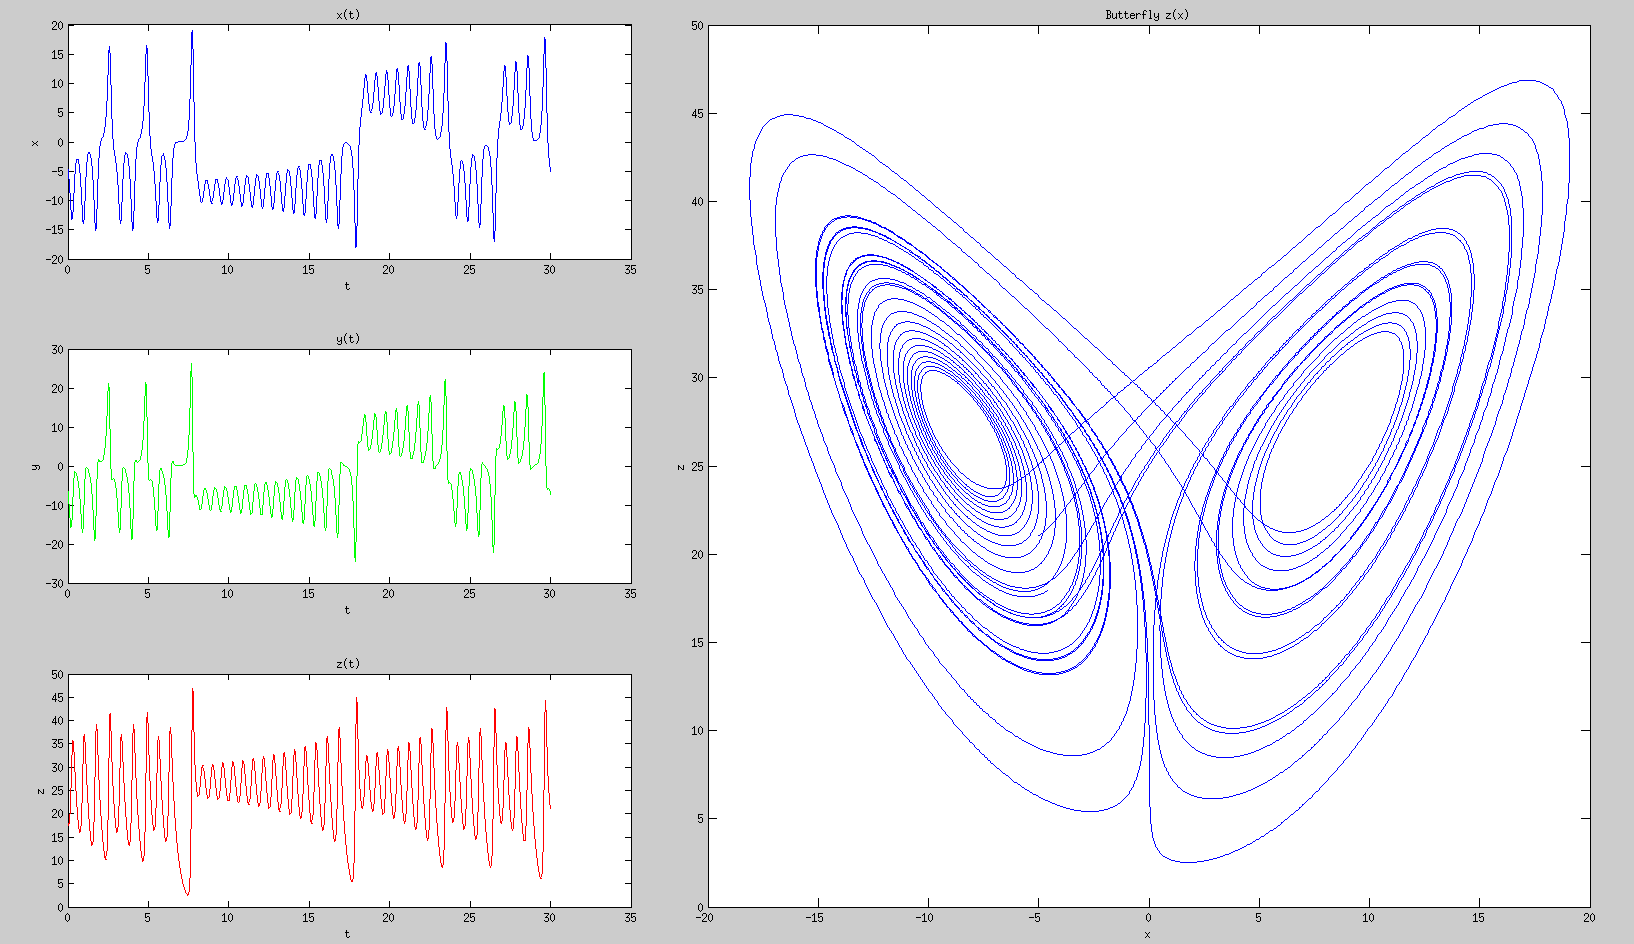
\includegraphics[width=16cm]{results.png}
   \caption{Reference run with RK4 and $\Delta_t = 10^{-3}$.}
\end{figure}

The results are not exactly the same but we have no information on the method used so I tend to trust more my Runge-Kutta 4 which converges to a fixed solution with $\Delta_t \leq 10^{-3}$.

\clearpage

\section{Data assimilation experiments}

In all this section I will use unless otherwise specified $\colbox{\Delta_t = 10^{-3}}$, $\colbox{P_b = diag(\sigma_b^2, \sigma_b^2, \sigma_b^2)}$, $\colbox{Q = diag(\sigma_q^2, \sigma_q^2, \sigma_q^2)}$ and $\colbox{R = diag(\sigma_r^2, \sigma_r^2, \sigma_r^2)}$. 
Our initial guess seems not so bad (background) so I fix $\colbox{\sigma_b^2 = 1m^2}$.
Model error variance is fixed at $\colbox{\sigma_q^2 = 0.01 m^2}$ because I trust my Runge-Kutta 4 discrete model and because the continuous model equations and parameters are exactly known. 
Measurement error variance strongly depends on sensor type and is initially fixed at $\colbox{\sigma_r^2 = 0.1m^2}$. 

\subsection{Question 8: All variables - All data - No noise}

The Kalman Filter algorithm is initialized with our background $\u^b$, observations are perfect and obtained by a previous run of Runge-Kutta 4 with the true initial condition $\u_0$. Here $\sigma_r^2$ should be zero but it has no real impact as it converges in very few iterations on the reference trajectory even with high values. This has been implemented in matlab file $question8.m$.

\vskip 0.3cm
Here is what I obtain for $T = 0.05s$ and $T = 3s$ :

\begin{figure}[H]
   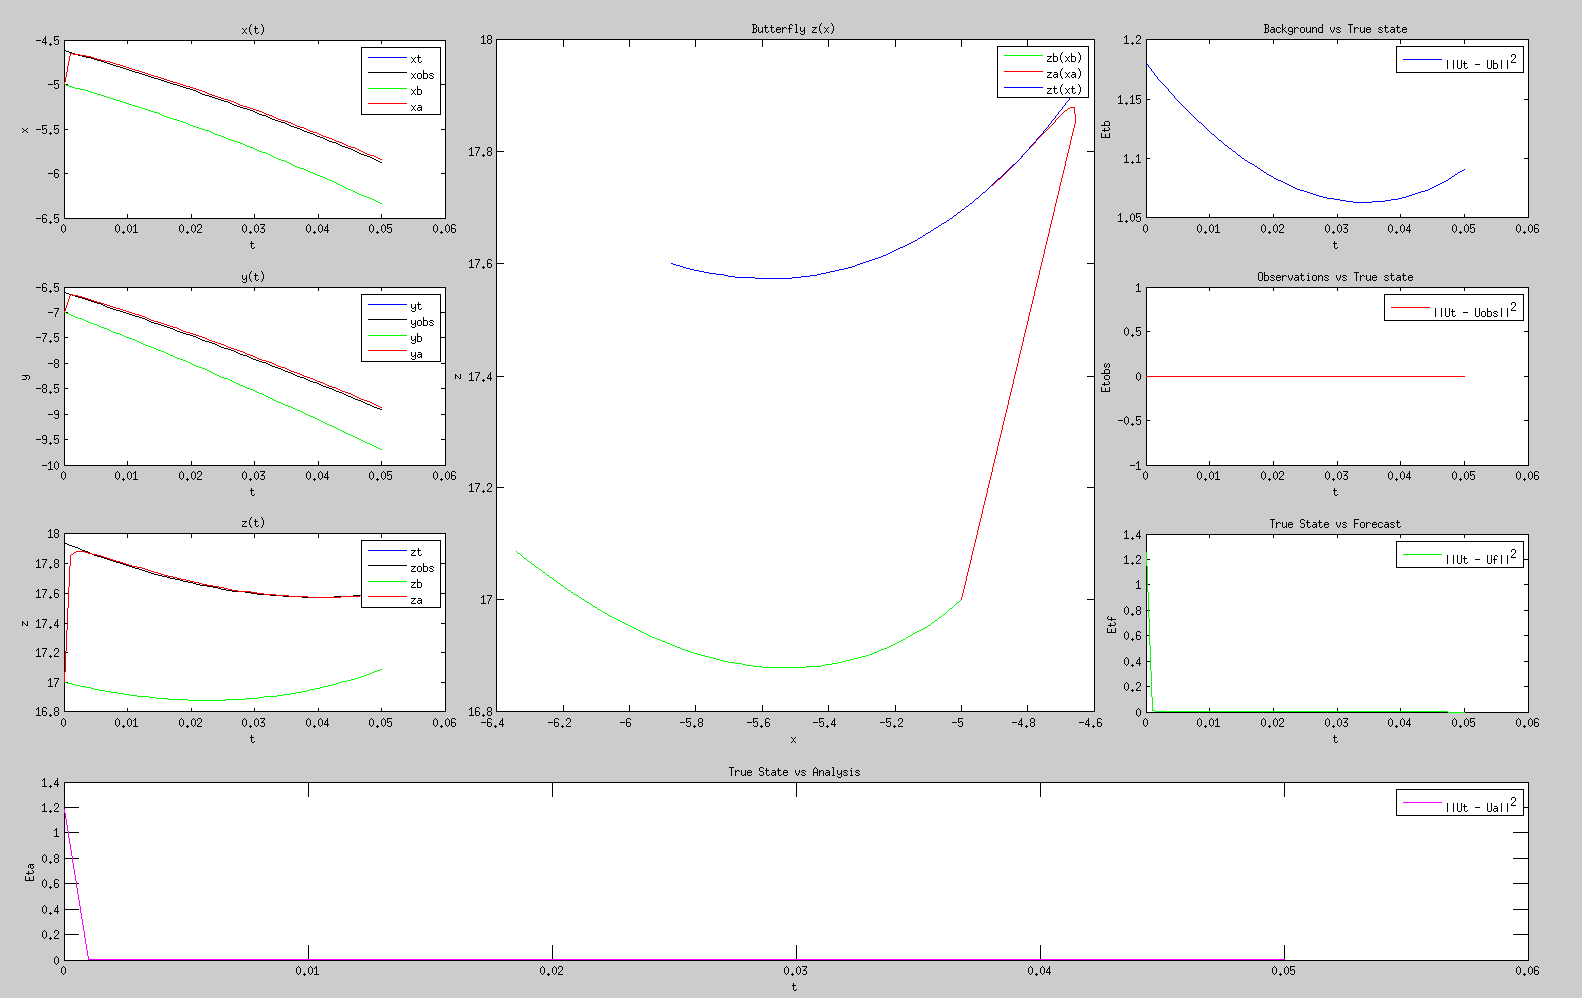
\includegraphics[width=16cm]{Q8a.png}
   \caption{Run with $T = 0.05s$.}
\end{figure}

On the 4 top leftmost plots, the true trajectory is in blue, the background trajectory in green, the analysis in red and the observations are in black. The four other plots are here for distance and error comparison. On the Butterfly plot and the "True State vs Analysis" plot we clearly see that \textbf{only 3 iterations are needed so that analysis and true state are perfectly matching}. All images in this report are available in  original size in the subfolder $img/$.

\begin{figure}[H]
   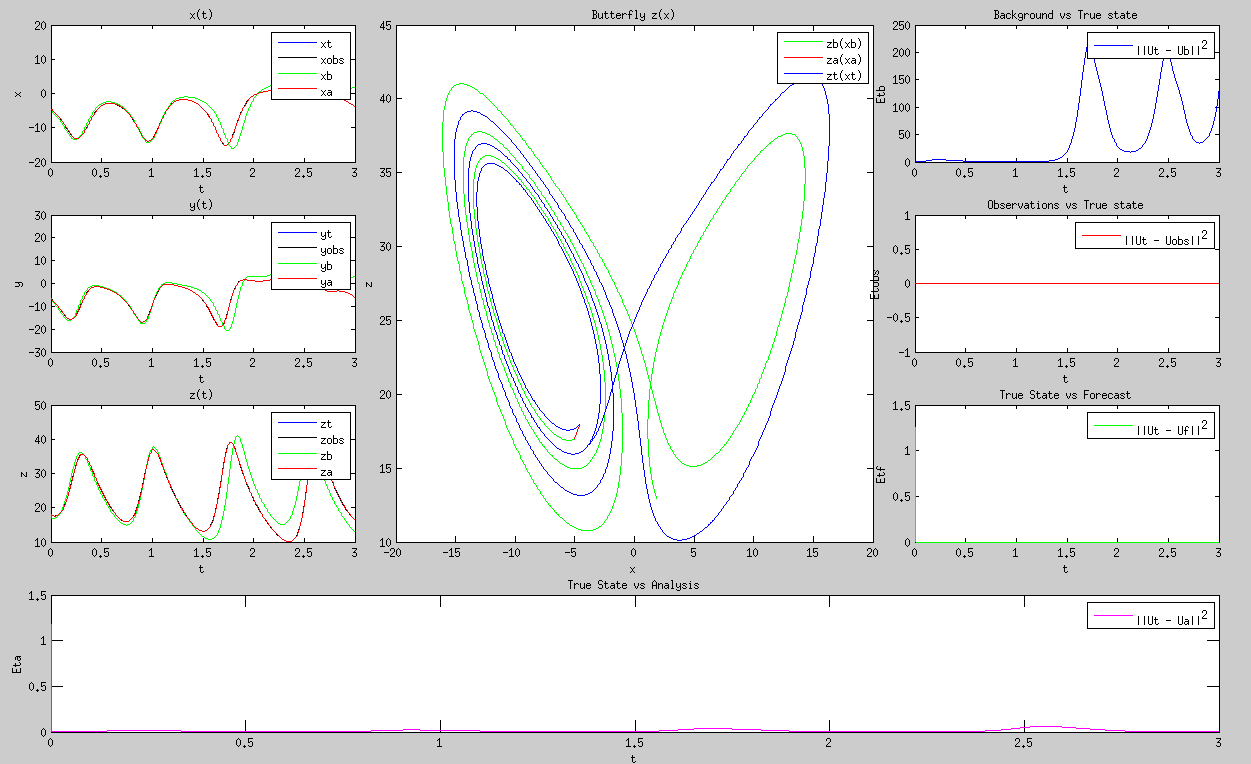
\includegraphics[width=16cm]{Q8b.png}
   \caption{Run with $T = 3s$.}
\end{figure}

With extended time view we can see that analysis and true state keep superimposed except at some critical regions around time $T = 1.3s$ and $T = 2.6s$ where the squared local error can go up to $0.1m^2$. This is nothing compared to what the background trajectory would give us at those points :  the "Background vs True State" graph gives us roughly a local squared error of respectively $200m^2$ and $180m^2$. \textbf{Thus the Kalman Filter implementation is stable and the twin experiment passes without any problem.}

\clearpage
\subsection{Question 9: Only one variable - All data - No noise}

\vskip 0.5cm

Now our sensor is broken and we can just observe one variable $x$. This can be simulated by configuring line $119$ of script $question8.m$ to true.
Here is what I obtain :

\vskip 0.5cm

\begin{figure}[H]
   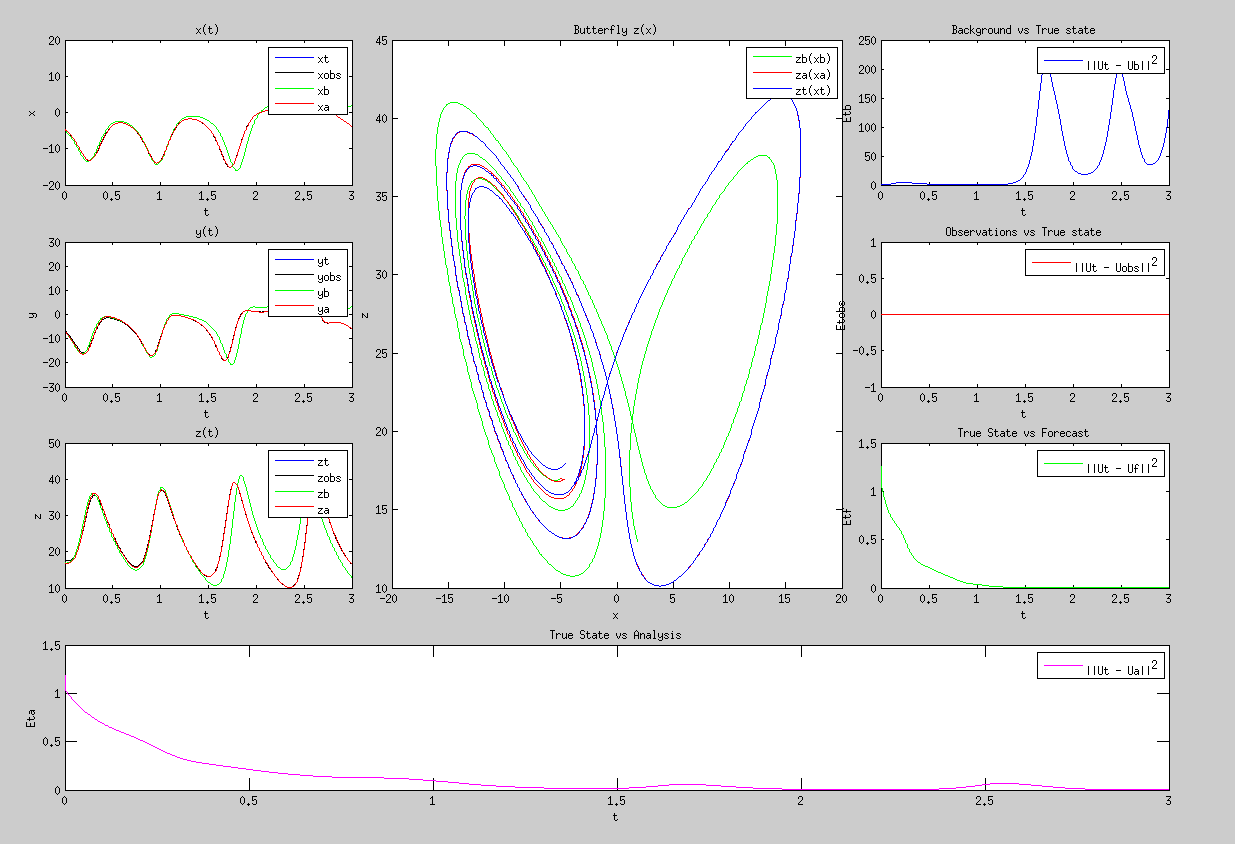
\includegraphics[width=16cm]{Q9.png}
   \caption{Only $x_{obs}$ is used and $T = 3s$.}
\end{figure}

\vskip 0.5cm

The results are not surprising, by looking at less variables \textbf{the convergence is just slowed down}, and the maximum error after $T=1.5s$ is comparable to the trajectory with all variables ($\norm{\u_b - \u_t}_{\infty}^2 \simeq 230 m^2$ vs $\norm{\u_a - \u_t}_{\infty}^2 \simeq 0.1 m^2)$. This is true because $y_a$ and $z_a$ are greatly impacted by variations of $x_a$ in the model (all variables are coupled). 

\clearpage
\subsection{Question 10: All variables - Some data - No noise}

In real life applications, all sensors do have a response time and can not give any feedback over a certain frequency. Instead of dealing with a frequency we can just drop out some measures every $K$ temporal steps corresponding to a duration without data $K \Delta_t$ defining this frequency.
This can be configured on line $120$ in the same matlab file as before as a ratio of available data $\xi \in\ ]0,1]$.

\vskip 0.3cm
\noindent Here are the results obtained for various values of $\xi$ :

\begin{figure}[H]
   \centering
   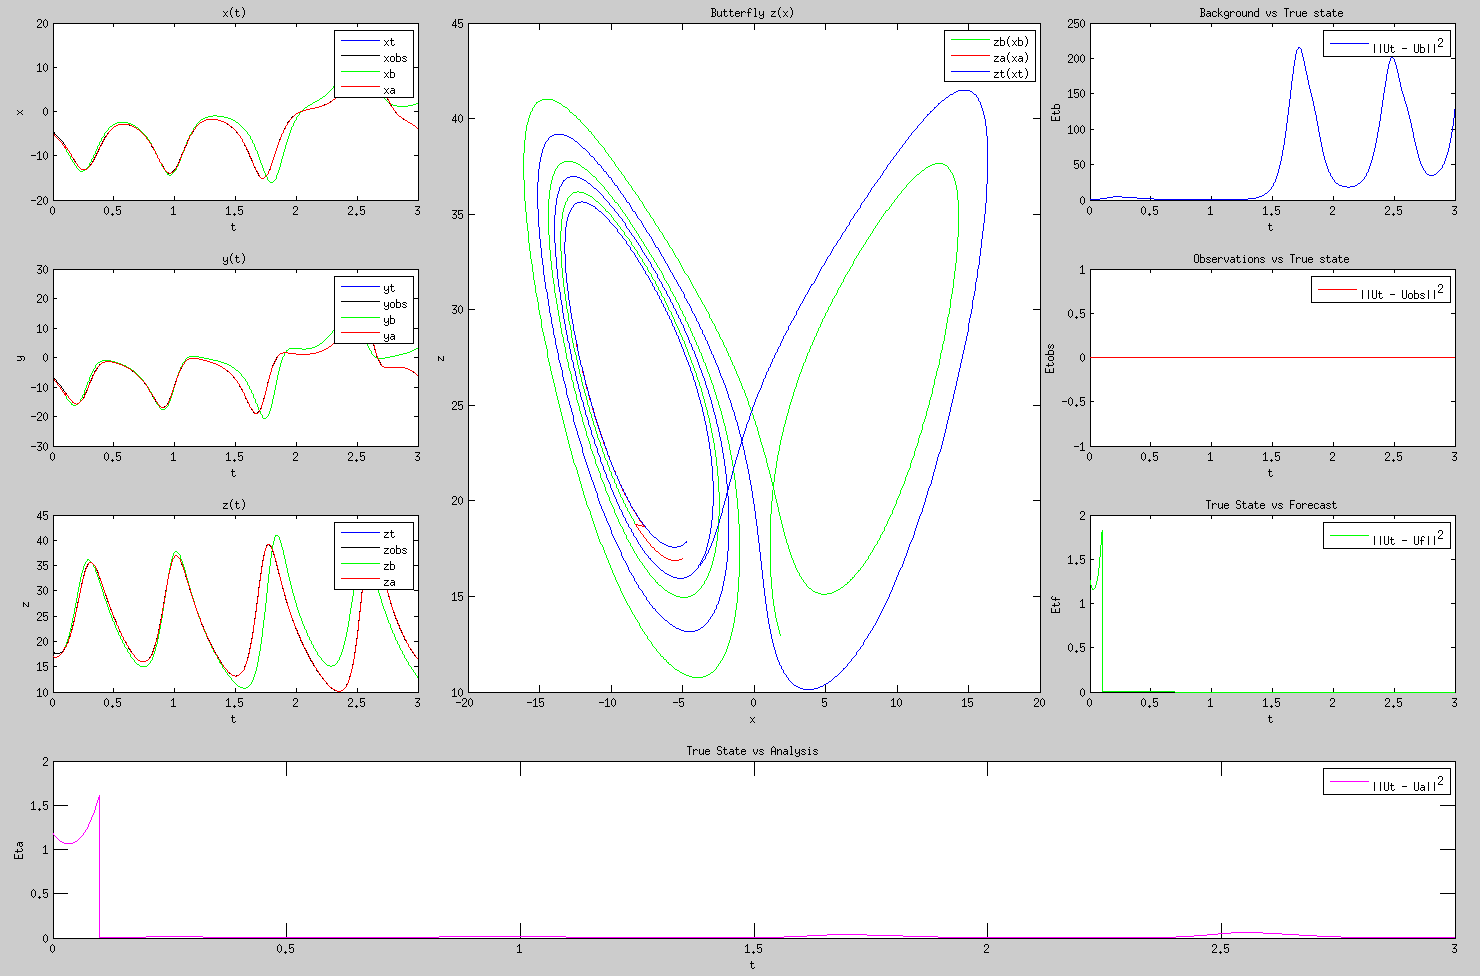
\includegraphics[width=12cm]{Q10a.png}
   \caption{$\xi = 0.1$}
\end{figure}

\begin{figure}[H]
   \centering
   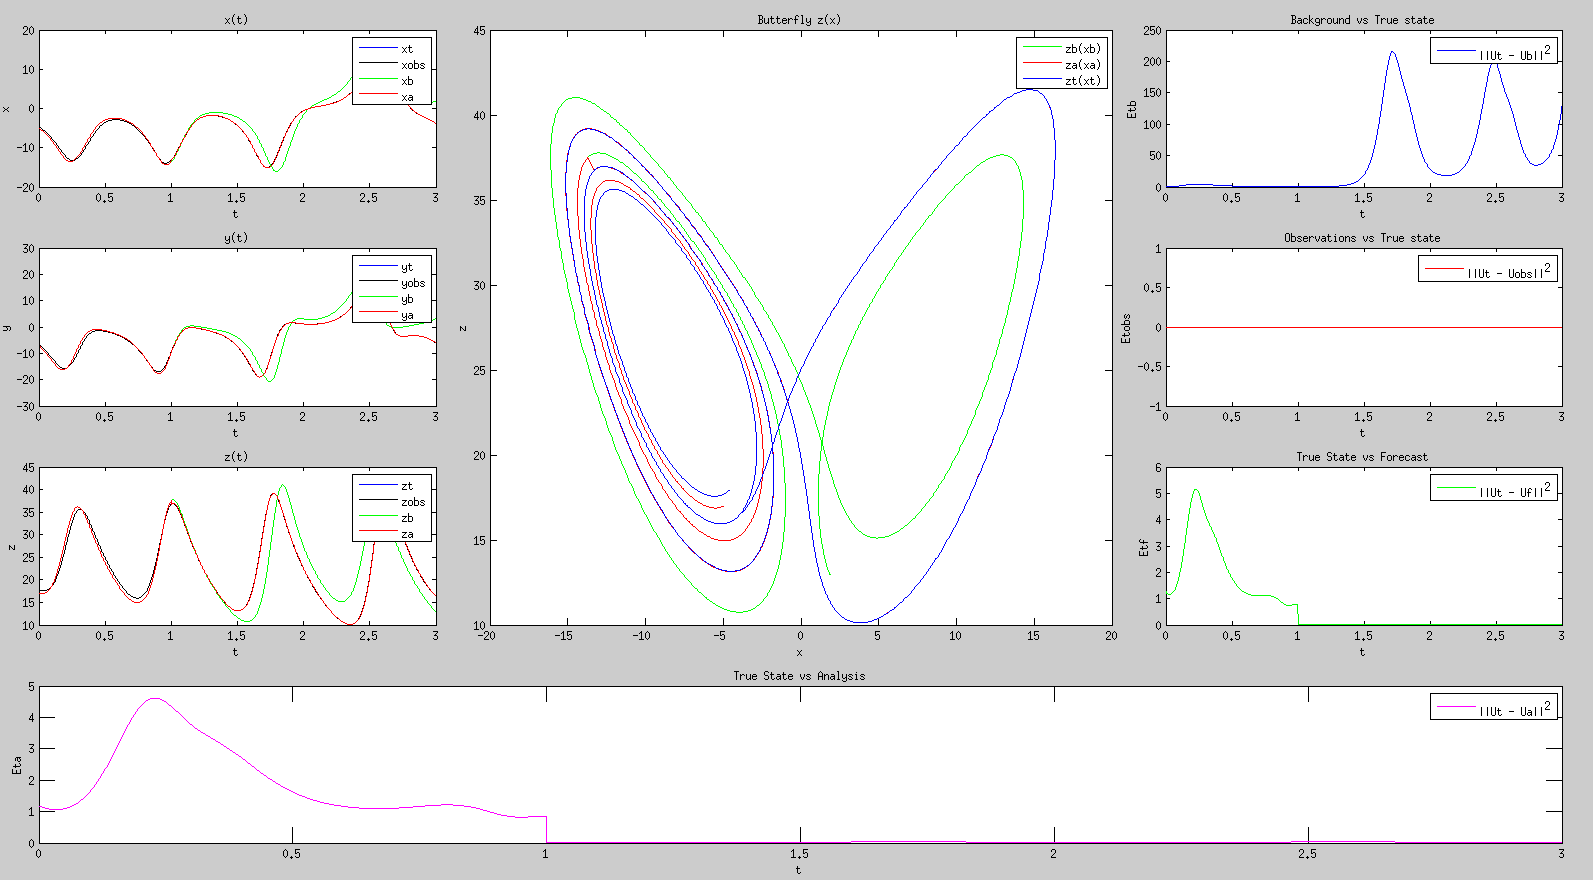
\includegraphics[width=12cm]{Q10b.png}
   \caption{$\xi = 0.01$}
\end{figure}

Without noise this parameter is not interesting because it \textbf{just delays the rapid convergence of the Kalman Filter with perfect observations} (3 steps) that we have seen before in question 8.

\clearpage
\subsection{Question 11: All variables - All data - Gaussian noise}

\vskip 0.3cm
Data extracted from sensors are never perfect so let us try to corrupt them with some zero mean Gaussian noise with variance $\sigma_e$. This can be changed on line $121$ and the measurement error variance $\sigma_r$ can be changed on line $91$ as well.

\subsubsection{Good sensor}

\vskip 0.3cm
In this section we have a very good and costly laser based position sensor with given worst $\sigma_r^2 = 10^{-2}m^2$ within estimated speed window. We generate noise with $\sigma_e = \sigma_q$ to mimic such a sensor.

\vskip 0.5cm
\begin{figure}[H]
   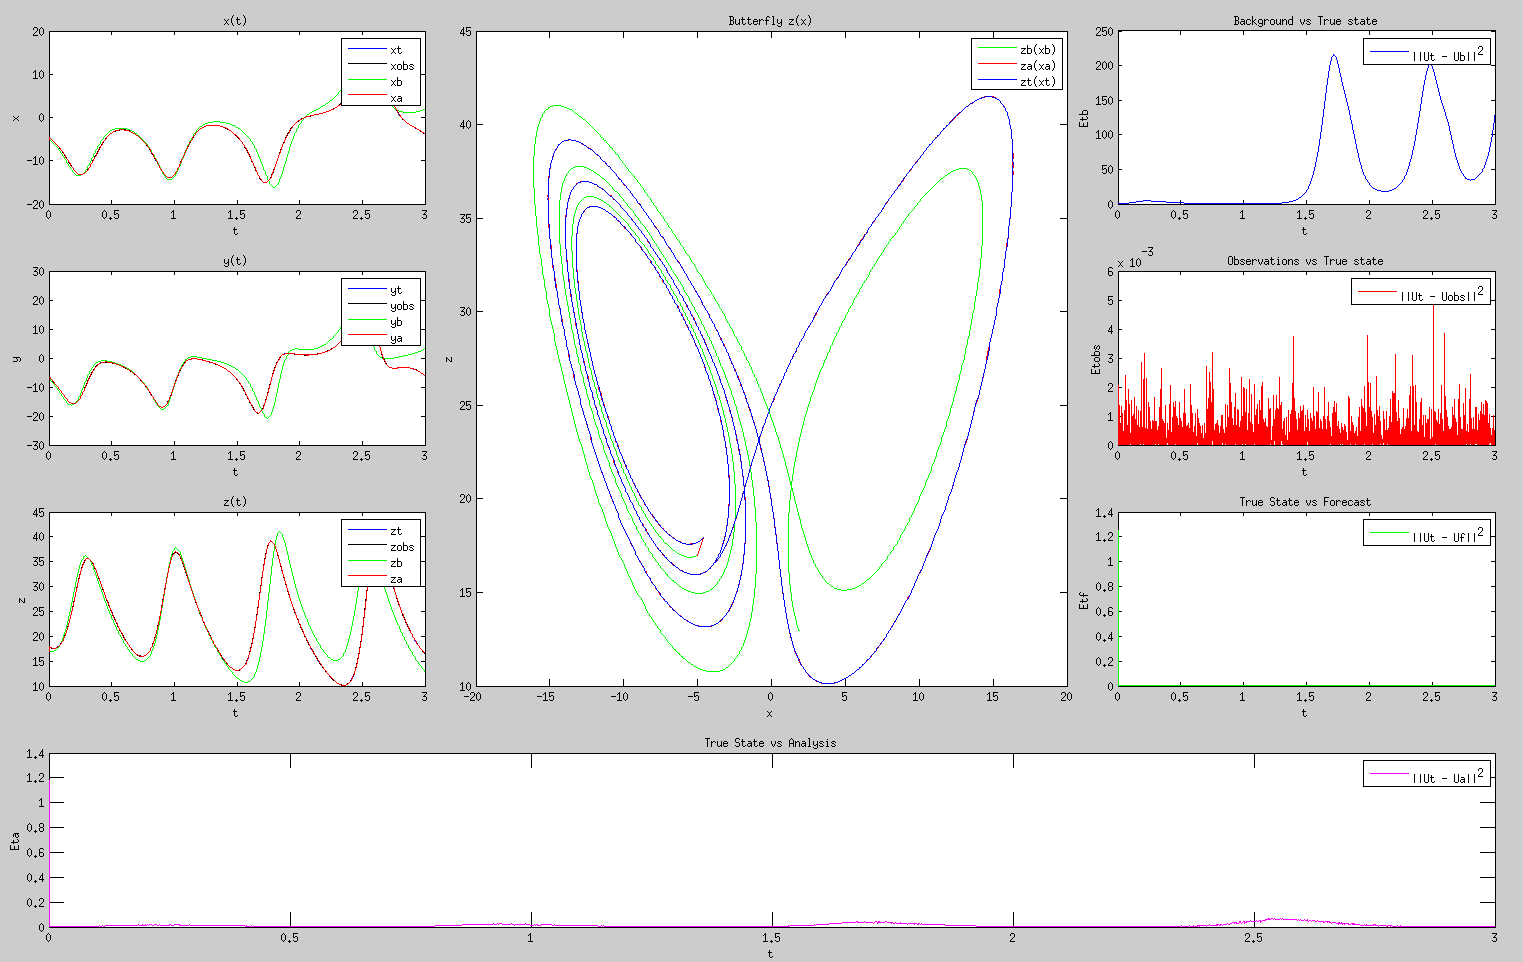
\includegraphics[width=16cm]{Q11a.png}
   \caption{$\sigma_e^2 = \sigma_r^2 = 0.01 m^2$}
\end{figure}

\vskip 0.5cm
As we could have expected we can barely see noise in the results, the Kalman Filter is still doing its job with those quite perfect input data !

\clearpage 
\subsubsection{Cheap sensor}

\vskip 0.3cm
Now we take a cheap real time segmentation based position retrieval technique with estimated worst $\sigma_r^2 = 0.5m^2$ within estimated background speed range. As before we generate noise with $\sigma_e = \sigma_q$ to simulate such incoming sensor data.

\vskip 0.5cm
\begin{figure}[H]
   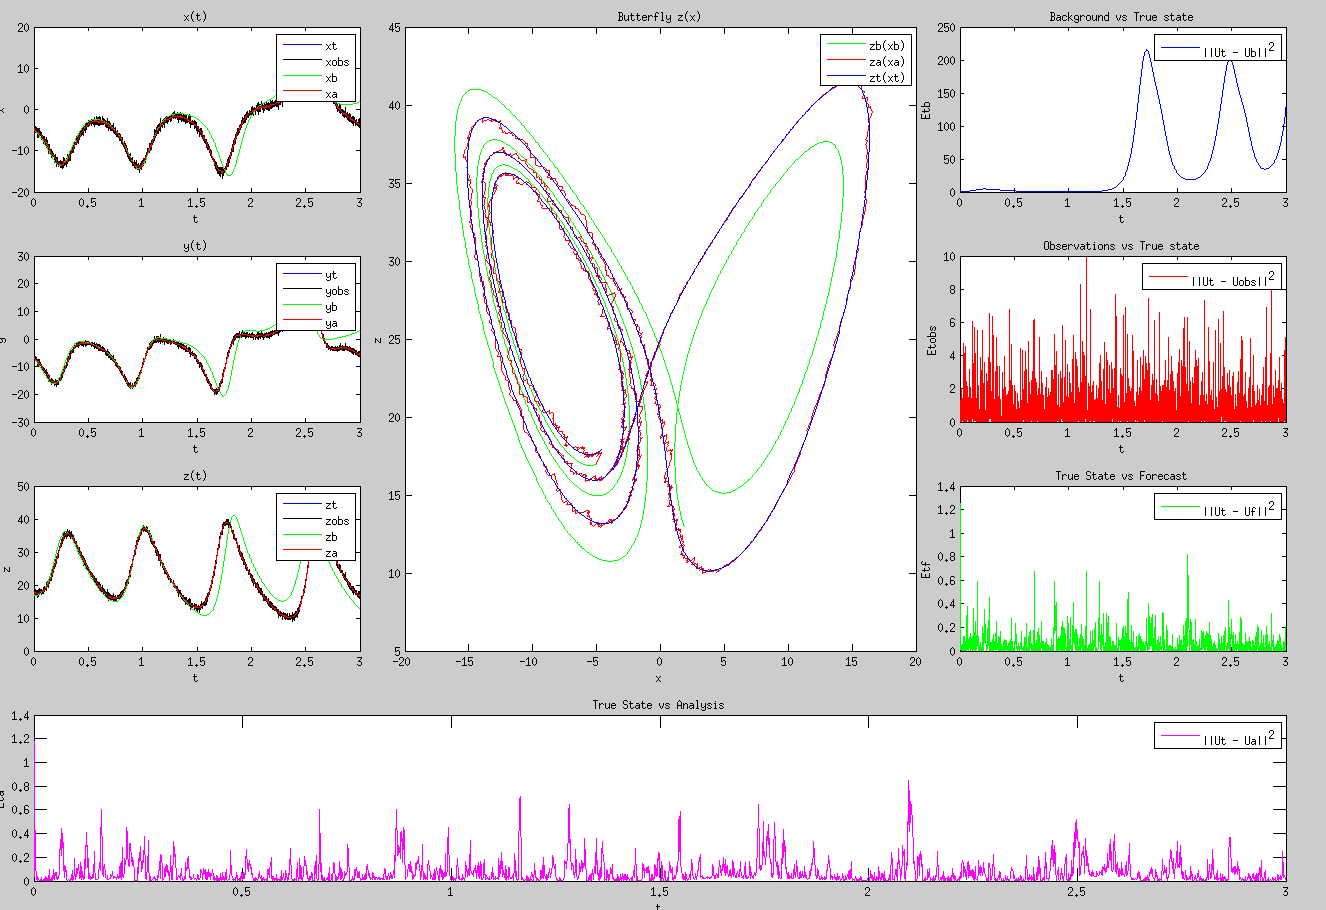
\includegraphics[width=16cm]{Q11b.png}
   \caption{$\sigma_e^2 = \sigma_r^2 = 0.5m^2$}
\end{figure}
\vskip 0.5cm

We really see that even if the sensor data are really noisy we can still extract a much better trajectory when compared to the background trajectory. 
\textbf{The Kalman Filter is really powerful for this application}, we can check it like before with $\norm{\u_b - \u_t}_{\infty}^2 \simeq 230 m^2$ vs $\norm{\u_a - \u_t}_{\infty}^2 \simeq 0.8 m^2$ if we exclude the initial background estimation.

\clearpage
\subsubsection{Badly calibrated sensor}

\vskip 0.3cm
Finally let us take some cheap sensor that is falsely advertised as very accurate with $\sigma_r^2 = 0.01 m^2$ like the first one but with real accuracy $\sigma_e^2 = 0.5m^2$.

\vskip 0.5cm
\begin{figure}[H]
   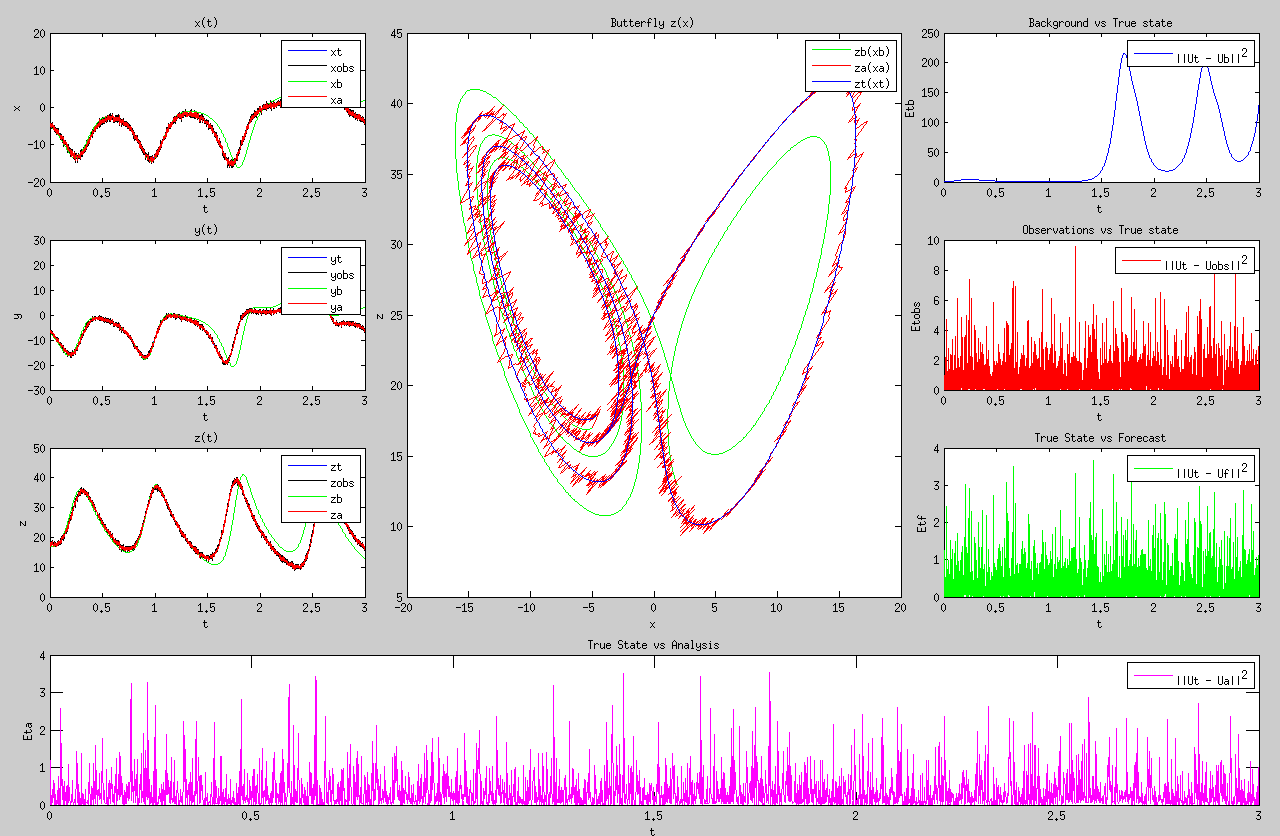
\includegraphics[width=16cm]{Q11c.png}
   \caption{$\sigma_e^2 = 0.5^2$ and $\sigma_r^2 = 0.01m^2$}
\end{figure}
\vskip 0.5cm

The algorithm now trust very noisy data and tries to get as close as it can to sensor sampled positions which results in noisy trajectories, the \textbf{model prevision is not taken much into account}.

\clearpage
\subsection{All variables - Some data - Gaussian noise}

For an overview of real life applications let us look at noisy sensor data that is not always available ($\xi < 1$) with our segmentation based sensor ($\sigma_r^2 = 0.5m^2$).

\begin{figure}[H]
    \centering
   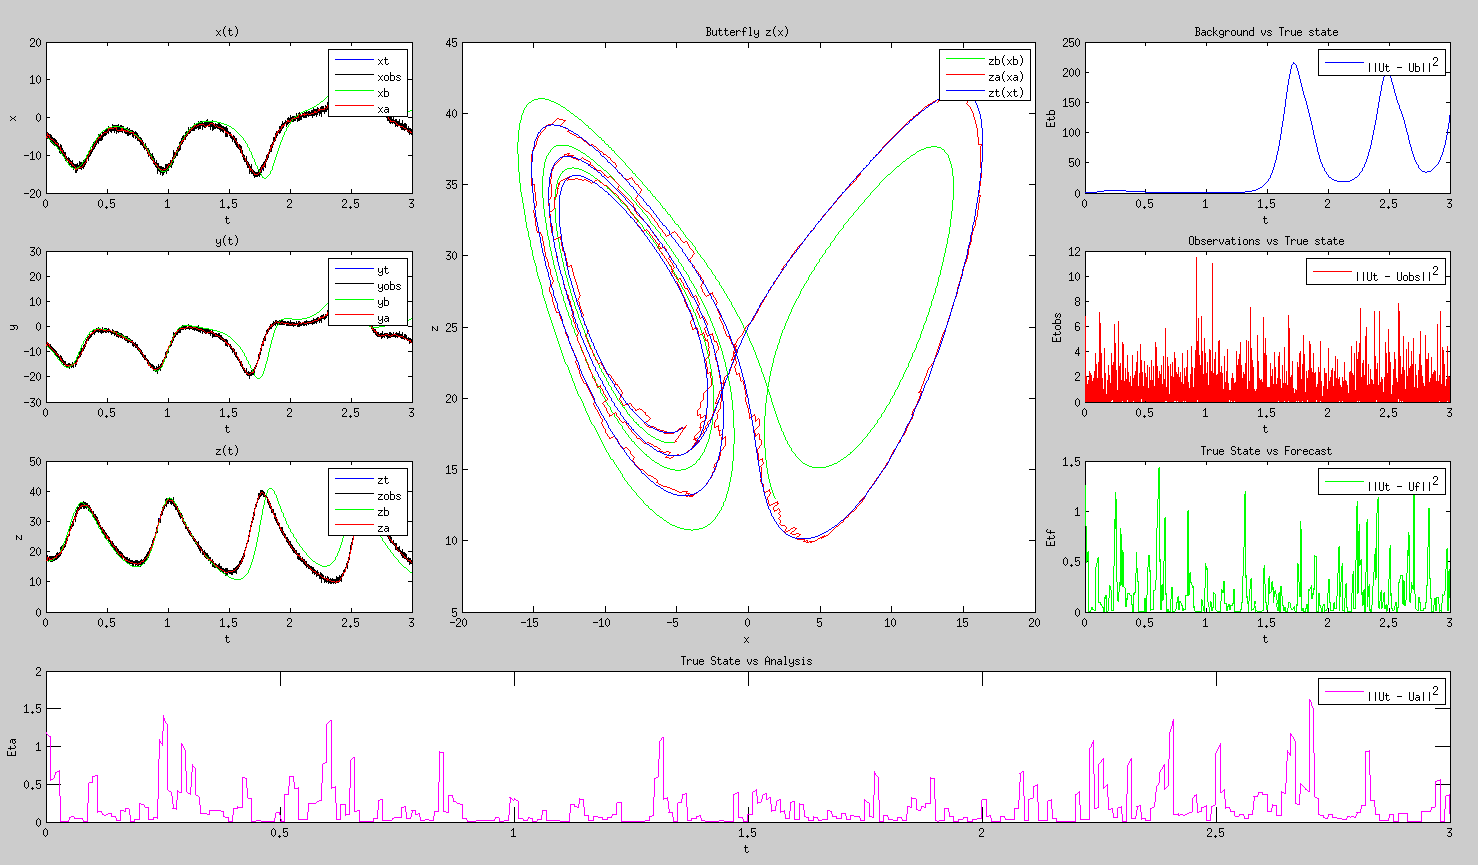
\includegraphics[width=14cm]{Q12a.png}
   \caption{$\sigma_e^2 = \sigma_r^2 = 0.5m^2$ and $\xi = 0.1$}
\end{figure}

\begin{figure}[H]
    \centering
   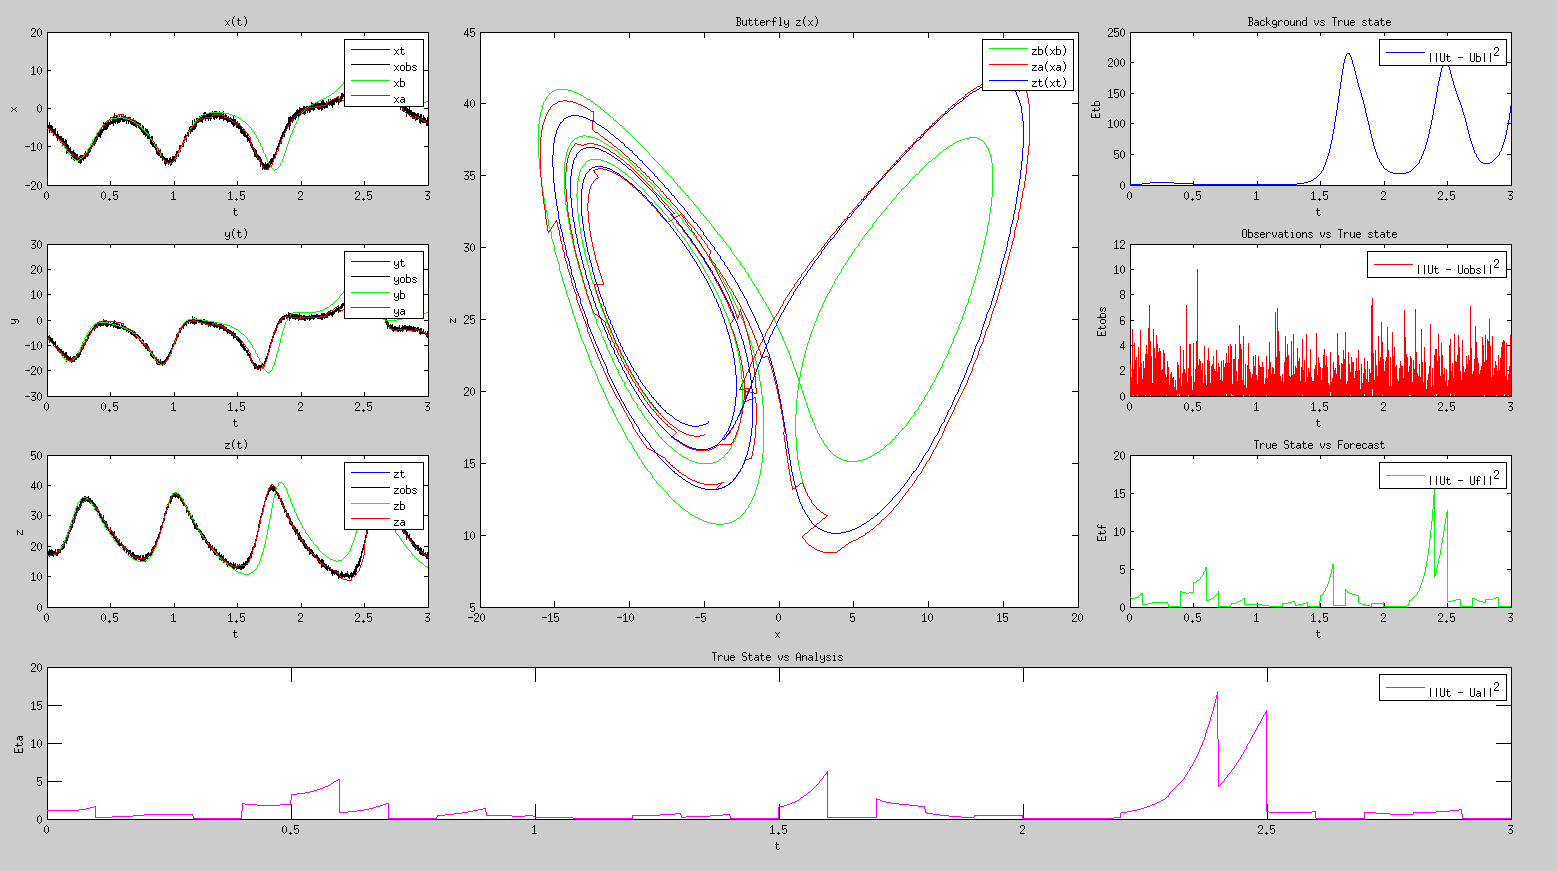
\includegraphics[width=14cm]{Q12b.png}
   \caption{$\sigma_e^2 = \sigma_r^2 = 0.5m^2$ and $\xi = 0.01$}
\end{figure}

\textbf{Even with only one percent of data we still have way better results than the original estimated background trajectory (by an order of magnitude of 10 in most critical regions)}. 

\clearpage
\subsection{Only one variable - Some data - Gaussian noise}

Finally let us observe just the system variable $x$ with exactly the two same set of parameters as before to see how the Kalman Filter will respond.

\begin{figure}[H]
    \centering
   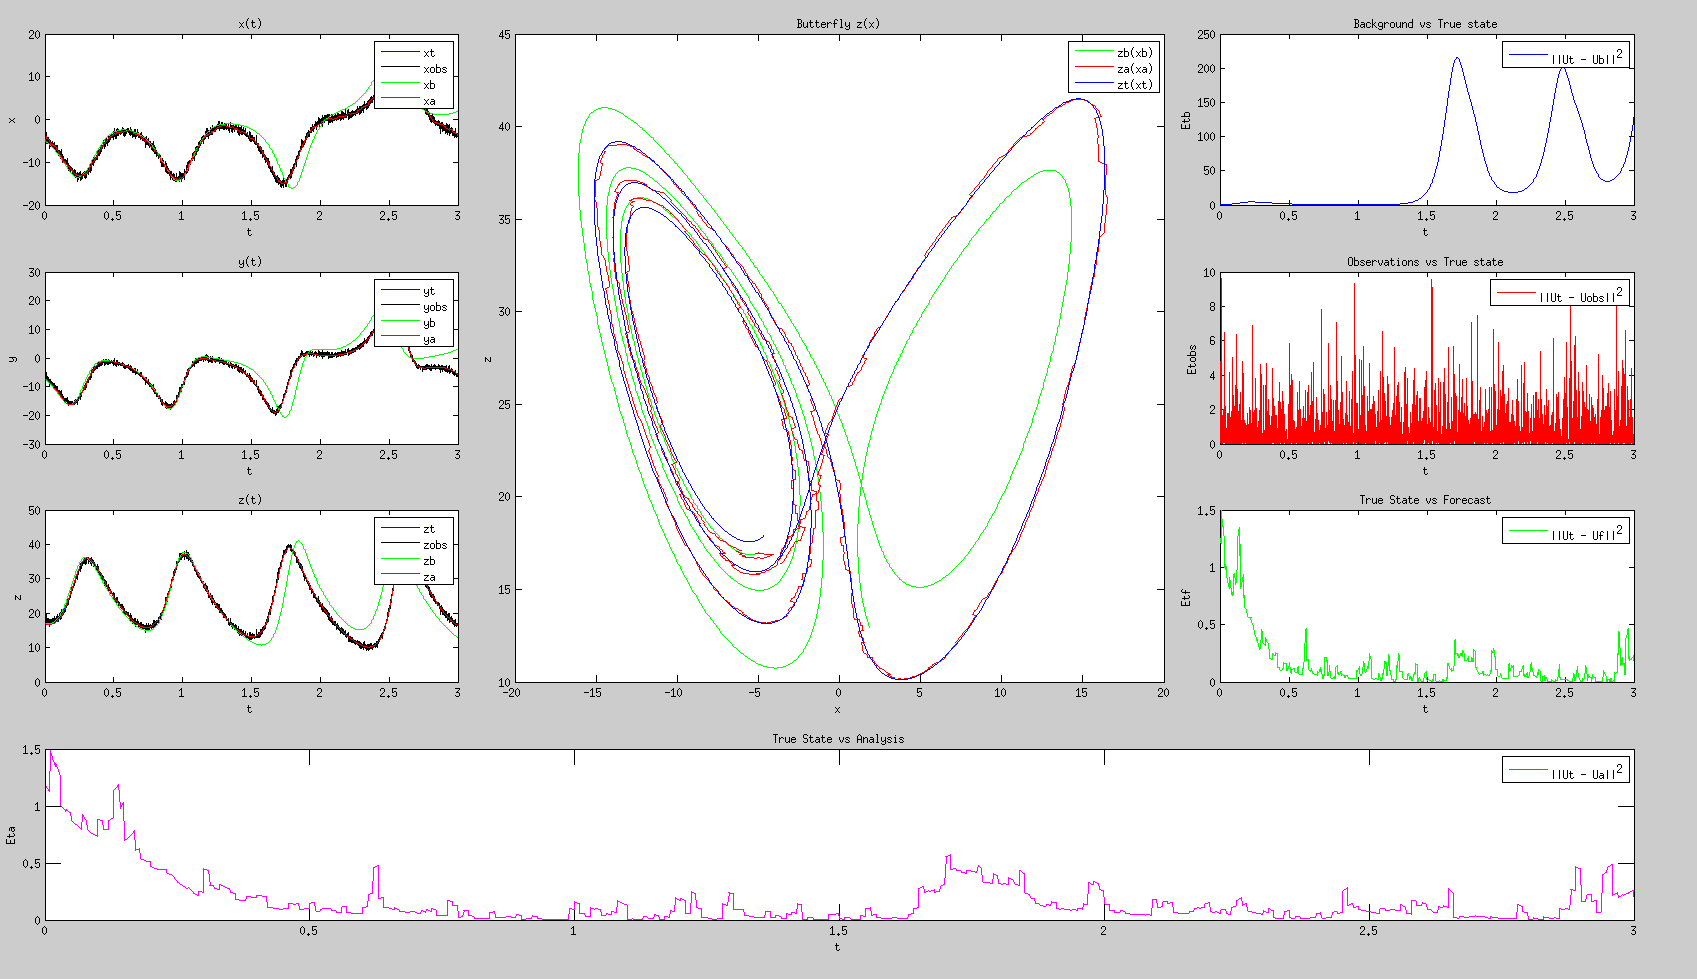
\includegraphics[height=7cm]{Q13a.png}
   \caption{Only $x^{obs}$ is used, $\sigma_e^2 = \sigma_r^2 = 0.5m^2$ and $\xi = 0.1$}
\end{figure}

With $10\%$ of very noisy data of only one variable results are really interesting ! Mean error between analysis and true state \textbf{really exhibits the power of Kalman filtering}.

\begin{figure}[H]
    \centering
   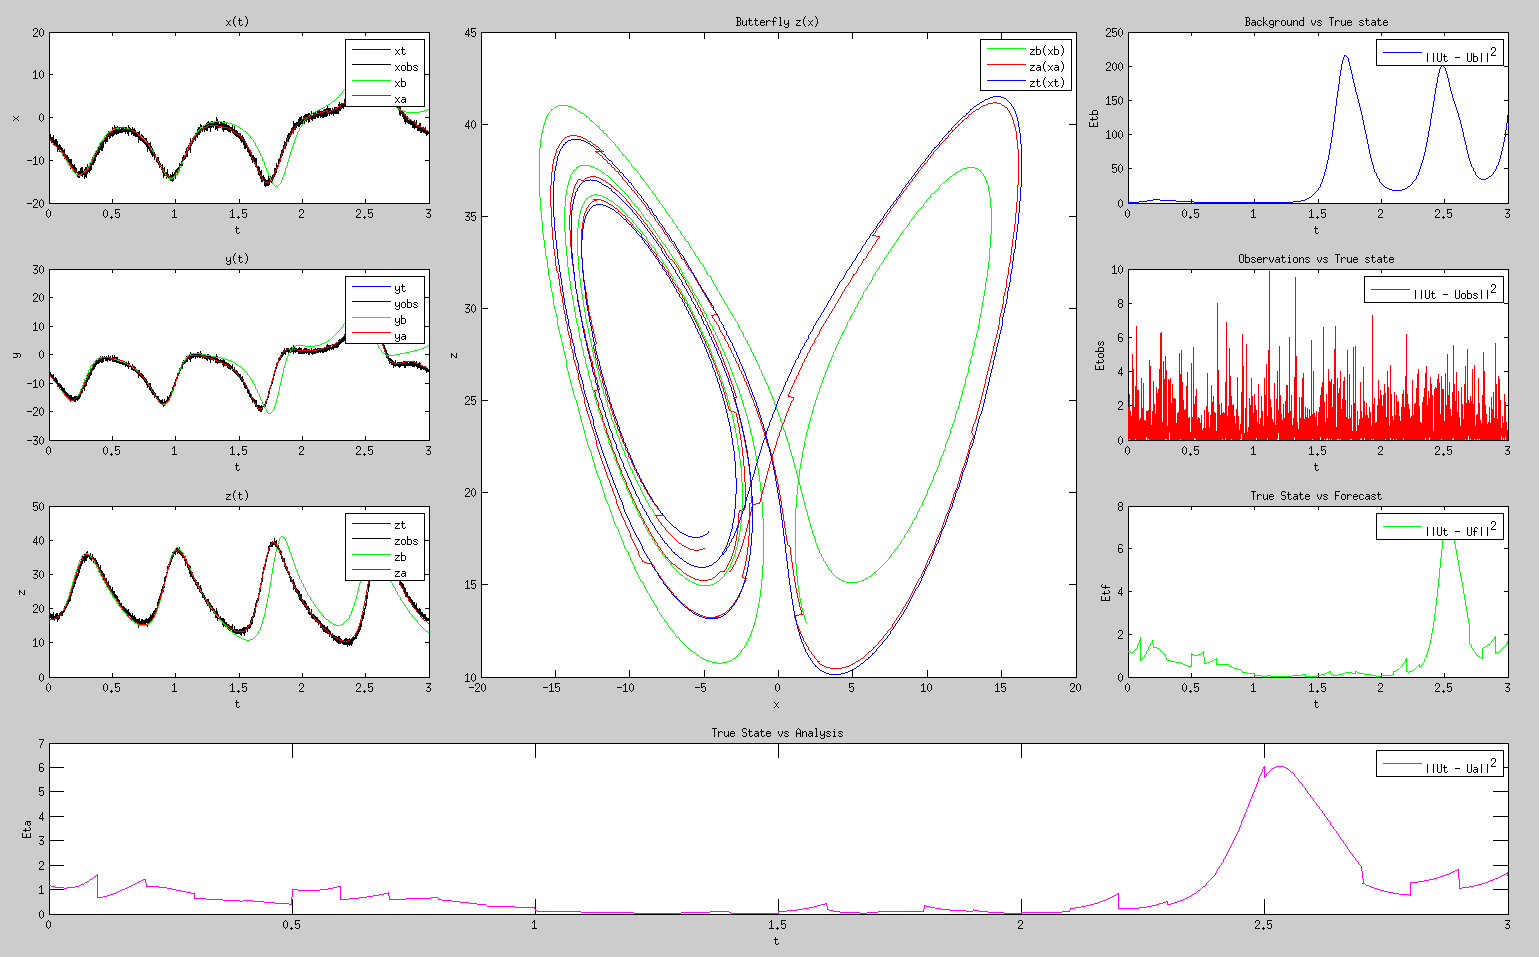
\includegraphics[height=8cm]{Q13b.png}
   \caption{Only $x^{obs}$ is used, $\sigma_e^2 = \sigma_r^2 = 0.5m^2$ and $\xi = 0.01$}
\end{figure}

\textbf{Here we have finally reached the limit of our filter}, there is not enough sensor data samples to sufficiently correct erroneous trajectories. We clearly see it around the critical region $t = 2.6s$. Needless to say, it is still far better than the original background trajectory without any corrections !

\clearpage
\section {Conclusion}

Implementing Kalman Filter is not so easy if the model is not linear. The model matrix $M_k$ was not easy to find. Even with local linearization and simple algorithms slightly more complicated than an Euler scheme, it rapidly becomes impossible to compute it by hand. I was often confronted to numerical instabilities (order of operations ...) or badly conditioned matrix and thus I lost much time in the code. But in the end all was working and I really experienced the power of data assimilation through Kalman filtering. I wanted to try the adjoint method by generating the adjoint RK4 code in C with tapenade but I gave up as time is too precious in this part of the year and this would have bring additional implementation considerations and bugs on the table.

\section {Source code and other files overview}

\begin{itemize}
    \item $Question6.m$ : Question 6 and 7 matlab implementation
    \item $Question8.m$ : Question 8 to 10 matlab implementation
    \item $Lorenz.m$ : Matlab implementation of the Lorenz Attractor
    \item $RK4.m$    : Matlab implementation of the Runge-Kutta 4 algorithm
    \item $RK4.c$    : C implementation of the Runge-Kutta 4 algorithm
    \item $RK4\_adjoint.c$    : C adjoint of the Runge-Kutta 4 algorithm generated by tapenade
    \item $model.mw$ : Maple computation of the model matrix
    \item $img/*.png$ : All the images used in this report

\end{itemize}

\end{document}
